\chapter{Deskriptive Analyse}

%Betrachtung was in den Daten enthalten ist (Geschlechter Verteilung, Alter, etc.)
In der durchgeführten wurden zu Beginn allgemeine Daten über die Teilnehmenden erhoben.
Die Informationen welche über die Teilnehmenden abgefragt worden sind, können in der Tabelle
\ref{tab:allgemeine_daten} eingesehen werden.

% \usepackage{float}
\begin{table}[h]
    \centering
    \begin{tabular}{|l|l|p{8cm}|}
        \hline
        \textbf{Variable} & \textbf{Frage} & \textbf{Bedeutung}\\
        \hline
        Geschlecht & QA1 & Welchem Geschlecht fühlt sich die Person angehörig\\
        Alter & QA2 & In Gruppen von 10 Jahren (Bsw. 16-25, 26-35, 66+)\\
        Kinder & QA3 & Hat die Person Kinder\\
        Vollzeit/Teilzeit & QA7 & Ist die Person in Vollzeit oder Teilzeit tätig\\
        Körperliche Beanspruchung & QA11 & Wie stark ist die körperliche Belastung der Arbeit\\
        Branche & QA12 & In welcher Branche ist die Person tätig\\
        Bereits 4TW & QA16 & Hat die Person bereits eine 4-Tage-Woche\\
        \hline
    \end{tabular}
    \caption{Allgemeine Daten der Teilnehmenden}
    \label{tab:allgemeine_daten}
\end{table}

Mit den Informationen kann zum einen eine allgemeine Aussage über die Gruppe der Teilnehmenden 
getroffen werden, als auch zu den Hypothesen im den Kapiteln \ref{chap:hypothese4},
\ref{chap:hypothese5} und \ref{chap:hypothese9}. Dadurch kann in diesem Kapitel auch betrachtet
werden, ob die Stichprobe repräsentativ ist und ob es besondere Ausprägungen in den Daten gibt.
 
Zu diesem Zweck wird mit der Betrachtung der Altersverteilung und des Geschlechts der Teilnehmenden begonnen.
Wie in Abbildung \ref{fig:altersverteilung} zu sehen ist, besteht die Gruppe der Teilnehmenden hauptsächlich aus Personen im Alter von 16 bis 35 Jahren.
Dabei ist die Gruppe der 16 bis 25 Jährigen leicht stärker vertreten als die Gruppe der 26 bis 35 Jährigen.

\begin{figure}
    \centering
    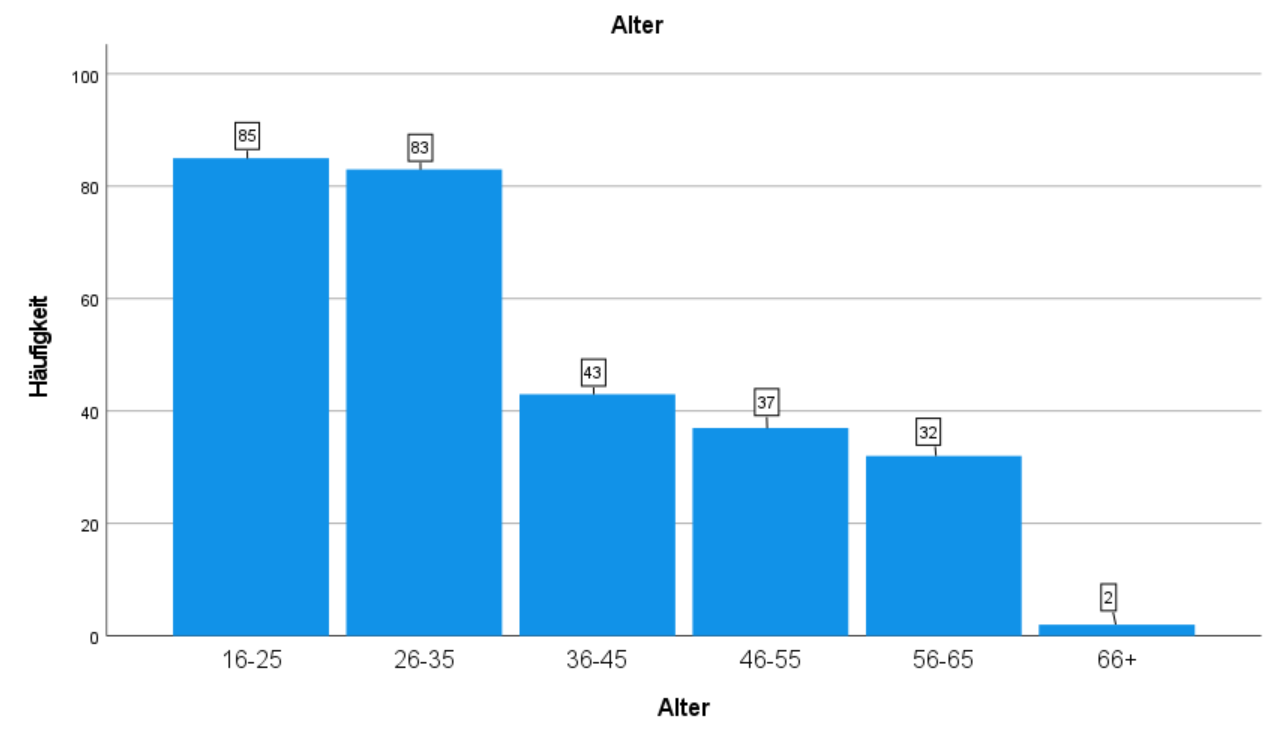
\includegraphics[width=0.8\textwidth]{04_Artefakte/01_Abbildungen/deskriptiv_alter.png}
    \caption{Altersverteilung der Teilnehmenden}
    \label{fig:altersverteilung}
\end{figure}

Bei den Geschlechtern sieht die Verteilung wie in Abbildung \ref{fig:geschlechterverteilung} dargestellt aus. Es gab mit 145 männlichen und 133 weiblichen Personen leicht
mehr Männer als Frauen in der Umfrage. Dazu kamen noch 3 Personen, die sich als divers identifiziert haben und 1 Person, die keine Angabe gemacht hat.

\begin{figure}
    \centering
    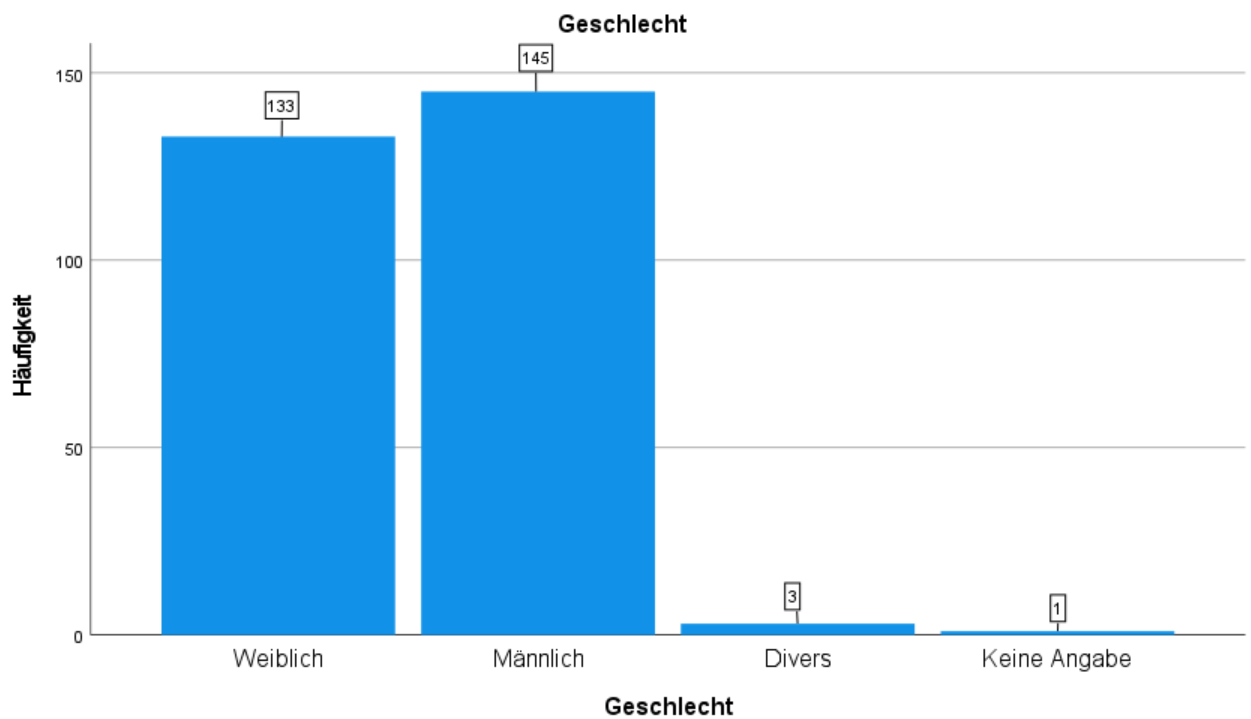
\includegraphics[width=0.8\textwidth]{04_Artefakte/01_Abbildungen/deskriptiv_geschlecht.png}
    \caption{Geschlechterverteilung der Teilnehmenden}
    \label{fig:geschlechterverteilung}
\end{figure}

